%% LyX 2.3.1-1 created this file.  For more info, see http://www.lyx.org/.
%% Do not edit unless you really know what you are doing.
\documentclass[english,hebrew]{article}
\usepackage[T1]{fontenc}
\usepackage[utf8]{inputenc}
\usepackage{babel}
\usepackage{amsmath}
\usepackage{graphicx}
\usepackage[unicode=true]
 {hyperref}
\begin{document}
\title{אבן נייר ומספרים ולטאה וספוק ובלבאוזר וצ'רמנדר וגרפים איזומורפיים}

\maketitle
אחד מהמשחקים הללו ש\textquotedblleft כולם מכירים\textquotedblleft{}
הוא \textquotedblright אבן, נייר ומספרים\textquotedblleft . החוקים
פשוטים: שני שחקנים עומדים ושרים לעצמם שיר בסגנון \textquotedblright אבן
נייר ומספרים המנצח מבין השניים אחת שתיים שלוש\textquotedblleft{} וחיש
קל שולחים יד קדימה באחת משלוש צורות: \textquotedblright אבן\textquotedblleft{}
)אגרוף(, \textquotedblright מספרים\textquotedblleft{} )אצבע ואמה זקורות(
ו\textquotedblleft נייר\textquotedblleft{} )כף יד פשוטה(. ואז... המשחק
מסתיים בתיקו כי שני השחקנים שלפו את אותו הדבר, ו\textquotedblleft המנצח
מבין השניים\textquotedblleft{} שבשם השיר נחשף במערומיו!

אבל אם השחקנים שלפו דברים שונים, המנצח נקבע על פי חוקים סבוכים שאפשר
לנסח כך: \textquotedblright אבן שוברת מספריים שגוזרים נייר שעוטפת
אבן\textquotedblleft . כלומר: כל \textquotedblright נשק\textquotedblleft{}
שאפשר לשלוף מנצח את אחד מהנשקים האחרים, ומפסיד לאחד מהנשקים האחרים.
אם שני השחקנים בוחרים נשק באקראי, אז הם ינצחו בשליש מהפעמים, יפסידו
בשליש מהפעמים ובשליש מהפעמים המשחק ייגמר בתיקו. כשמשחקים יותר מפעם
אחת ברצף כבר נכנס לתמונה מרכיב פסיכולוגי מעניין - קשה לשחקנים \textquotedblright להגריל
באקראי\textquotedblleft{} נשק בראש, כך שכל שחקן משחק באופן מוטה; מה
האסטרטגיה שכדאי לשחקן לאמץ כדי לנצח כמה שיותר פעמים? על זה אני לא
הולך לדבר הפעם, אבל זה תחום מגניב בפני עצמו.

לא מזמן הילד בן ה-{\beginL 5\endL} שלי סיפר לי על החידושים האחרונים
בעולם האבן-נייר-ומספריים: מתברר שאצלם בגן יש נשקים נוספים שכוללים
)בין היתר( \textquotedblright בור\textquotedblleft , \textquotedblright פצצה\textquotedblleft ,
\textquotedblright קשת\textquotedblleft , \textquotedblright רובה\textquotedblleft{}
וגם \textquotedblright פיל\textquotedblleft{} ו\textquotedblleft תרנגולת\textquotedblleft{}
עם חוקים סבוכים מאוד של מי מנצח את מי. הבעיה עם החוקים השרירותיים
שהמציאו באותו גן היא שהם \textbf{מוטים} לטובת נשקים מסויימים - למיטב
זכרוני \textquotedblright בור\textquotedblleft{} מנצח כמעט כל דבר שם.
מה שהיינו \textbf{רוצים} שיקרה, אם אנחנו רוצים משחק מעניין, הוא שכל
נשק ינצח \textbf{בדיוק} חצי מהנשקים האחרים, ויפסיד לחצי מהנשקים האחרים,
גם בגרסאות המוכללות.

אם יש ארבעה נשקים, קל לראות שזה בלתי אפשרי: אם נבחר את אחד מהנשקים,
נותרו לנו {\beginL 3\endL} אחרים. מכיוון ש-{\beginL 3\endL} הוא מספר
אי זוגי, אי אפשר לחלק אותו ל-{\beginL 2\endL}; אי אפשר שהנשק שלנו
ינצח \L{$1.5$} מהנשקים ויפסיד ל-\L{$1.5$} מהנשקים. אם כן, כדי שמשחק
\textquotedblright אבן נייר ומספריים מוכלל\textquotedblleft{} יעבוד,
הכרחי שמספר הנשקים בו יהיה \textbf{אי זוגי}.

מכאן אנחנו מקבלים שההכללה הראשונה של אבן נייר ומספריים צריכה להיות
עבור {\beginL 5\endL} נשקים. הכללה מוכרת שכזו נקראת \textquotedblright אבן-נייר-מספרים-לטאה-ספוק\textquotedblleft{}
והיא \L{\href{http://www.samkass.com/theories/RPSSL.html}{הומצאה}}
בידי סם קס וקרן ברילה ואחר כך הופיעה בתוכנית הטלוויזיה \textquotedblright המפץ
הגדול\textquotedblleft{} כך שעכשיו כל היקום מכיר אותה. מה זו לטאה אנחנו
יודעים, ומחווים אותה באמצעות הצמדת אצבעות לאגודל בצורה שמזכירה ראש
של לטאה; \textquotedblright ספוק\textquotedblleft{} הוא הדמות של לאונרד
נימוי מתוכנית הטלוויזיה \L{Star Trek}. ספוק הוא חצי וולקני, כלומר
שייך לגזע חייזרים ששם דגש על לוגיקה ומחווה שלום בעזרת פיצול אצבעות
)מחווה שלאונרד נימוי עצמו המציא, בהשראת ברכת הכוהנים(.

\L{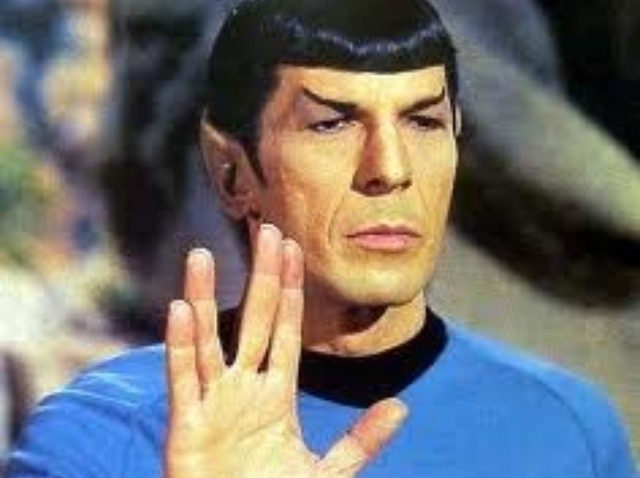
\includegraphics{C:/Users/gadia/Dropbox/Websites/blog/assets/img/2020/08/spock}}

הנשקים מתנהגים כך: אבן-נייר-מספרים מתנהגים כמקודם זה עם זה; לטאה מנצחת
את ספוק )\textquotedblleft מרעילה אותו\textquotedblleft ( ואת הנייר
)\textquotedblleft אוכלת אותו\textquotedblleft (, אבל מפסידה לסלע
ולמספריים שמחסלים אותה בצורה די בנאלית. ספוק לעומת זאת יודע לפצפץ
את הסלע והמספריים אבל הנייר מבלבל אותו )כנראה כתוב בצד אחד של הנייר
\textquotedblright מה שכתוב בצד השני הוא שקר\textquotedblleft{} ובצד
השני כתוב \textquotedblright מה שכתוב בצד השני הוא אמת\textquotedblleft (.
את כל זה אפשר להציג בדיאגרמה הבאה:

\L{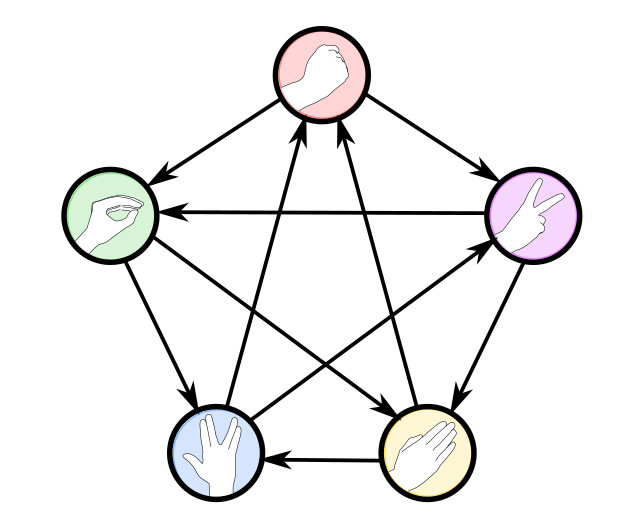
\includegraphics{C:/Users/gadia/Dropbox/Websites/blog/assets/img/2020/08/rpsls}}

כאן מתעוררת בי כבר שאלה - מה זה בעצם אומר, שהמשחק הזה \textquotedblright הומצא\textquotedblleft{}
בידי סם קס וקרן ברילה? מה שהם בוודאי המציאו זה את \textbf{השמות} של
הנשקים החדשים )לטאה וספוק(, את \textbf{מחוות הידיים} בשבילם ואת \textbf{הנימוקים}
לכך שנשק אחד מנצח את השני. כל אלו הם דברים חשובים ביותר - בלעדיהם
לא נזכור את חוקי המשחק והוא לא ייראה לנו מגניב. אבל מבחינה \textbf{מתמטית}
הם לא רלוונטיים - אלו \textquotedblright רק\textquotedblleft{} סימונים
וסיפורים, והמתמטיקה מתעניינת בהפשטה - במה שנשאר אחרי שמסירים את הדברים
הללו. כמו שהמתמטיקה מתעסקת בשאלה \textquotedblright כמה זה {\beginL 2+3\endL}\textquotedblleft{}
שהיא הפשטה של שאלות קונקרטיות כמו \textquotedblright כמה זה שני תפוחים
ועוד שלושה תפוחים\textquotedblleft{} או \textquotedblright לאיזו קומה
נגיע אם אנחנו בקומה {\beginL 2\endL} ואנחנו עולים שלוש קומות\textquotedblleft .

אחרי ההפשטה, מה שנשאר לנו מהמשחק הוא זה:

\L{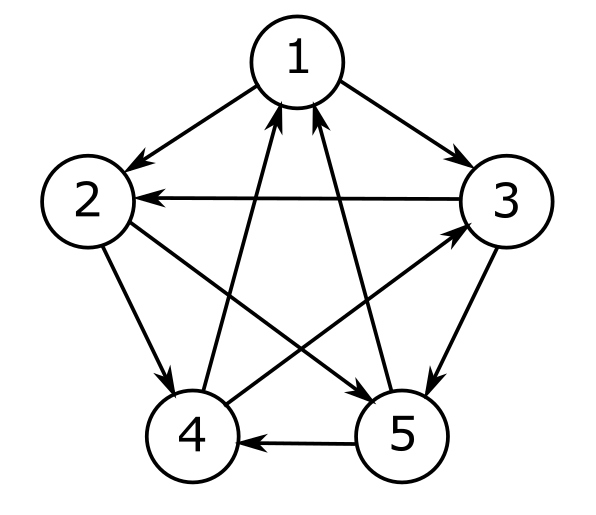
\includegraphics{C:/Users/gadia/Dropbox/Websites/blog/assets/img/2020/08/RPS5_RAW.PNG}}

ציור כזה נקרא \textbf{גרף}. יש בו שני סוגים של דברים: \textquotedblright עיגולים\textquotedblleft{}
ו\textquotedblleft חצים\textquotedblleft . לעיגולים קוראים \textbf{צמתים}
ולחצים קוראים \textbf{קשתות}. ברמה הכי פורמלית של העניין, גרף הוא
קבוצה \L{$V$} של צמתים )במקרה שלנו, הצמתים הם המספרים מ-{\beginL 1\endL}
עד {\beginL 5\endL}( ועוד קבוצה \L{$E$} של קשתות, כשכל קשת היא זוג
של צמתים, עם חשיבות לסדר: \L{$e=\left(v,u\right)$}, ולפעמים מסמנים
פשוט \L{$v\overset{e}{\to}u$}.

גרף כזה הוא נקודת ההתחלה שלנו כשאנחנו באים לבנות משחק \textquotedblright אבן-נייר-ומספריים\textquotedblleft{}
מוכלל עבור חמישה נשקים - אנחנו לוקחים את הגרף, נותנים שם לכל צומת,
ואז עבור כל קשת \L{$v\overset{e}{\to}u$} אנחנו ממציאים הסבר למה \L{$v$}
מנצח את \L{$u$}.

בואו נעשה את זה בפועל, באמצעות \textbf{פוקימונים}. הרעיון בפוקימונים
הוא שלכל פוקימון יש \textquotedblright טיפוס\textquotedblleft{} - יש
פוקימוני אש, פוקימוני מים וכדומה. חלק מסוגי הפוקימונים פגיעים להתקפות
מסוג פוקימונים אחר - למשל, פוקימון אש פגיע להתקפות מים. כבר במשחק
הפוקימונים הראשון, שלושת הפוקימונים \textquotedblright הבסיסיים\textquotedblleft{}
ביותר - צ'רמנדר עבור \textquotedblright אש\textquotedblleft , סקווירטל
עבור \textquotedblright מים\textquotedblleft{} ובלבאוזר עבור \textquotedblright עשב\textquotedblleft{}
- נבחרו כדי לקיים יחסים כמו באבן נייר ומספריים: אש מנצחת עשב שמנצח
מים שמנצחים אש:

\L{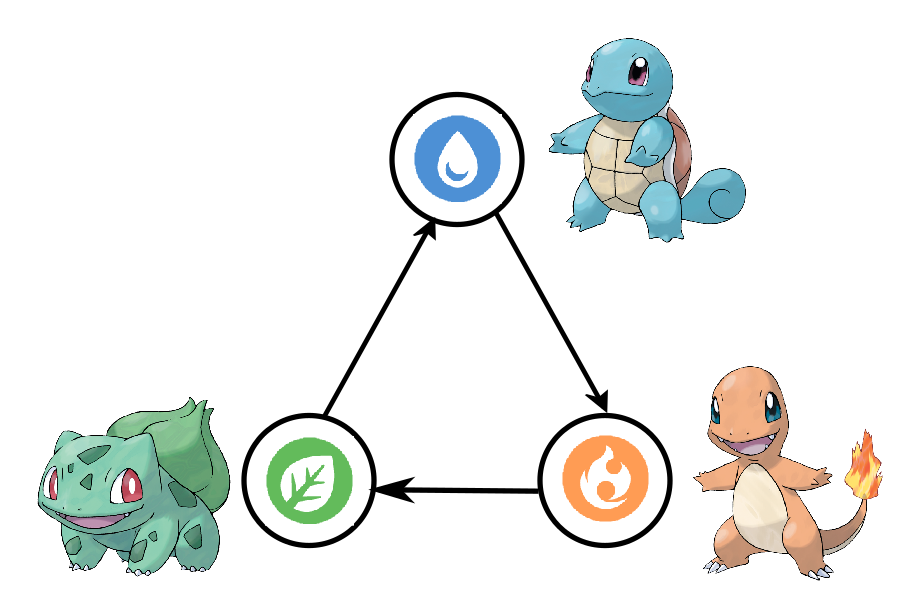
\includegraphics{C:/Users/gadia/Dropbox/Websites/blog/assets/img/2020/08/RPS-3Pokemon.PNG}}

אני רוצה להכליל את זה עבור חמישה פוקימונים, כך שכל פוקימון פגיע לשניים
אחרים, ושניים אחרים פגיעים אליו. לרוע המזל, המבנה של משחק הפוקימונים
הוא כזה שלא ניתן \textbf{להרחיב} את השלשה של אש-מים-עשב כדי להשיג
את זה )אין עוד טיפוסי פוקימונים שמשתלבים בצורה סימטרית עם שלושת אלו(
אבל אם אחליף את \textquotedblright מים\textquotedblleft{} ב\textquotedblleft קרח\textquotedblleft{}
)שמיוצג על ידי הפוקימון לאפרס שהוא פוקימון משולב של מים/קרח( ואוסיף
פנימה את פוקימון ה\textquotedblleft אדמה\textquotedblleft{} דיגלט ואת
פוקימון ה\textquotedblleft סלע\textquotedblleft{} אוניקס, אני אוכל
לקבל את משחק האבן-נייר-ומספרים מוכלל שרציתי.

בואו ניקח את הגרף שהראיתי קודם:

\L{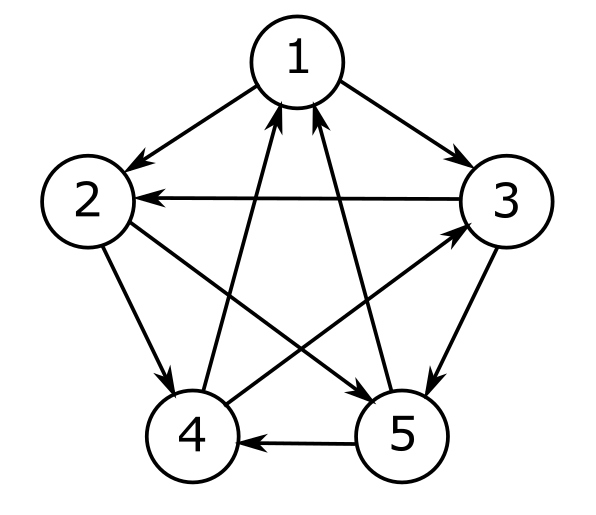
\includegraphics{C:/Users/gadia/Dropbox/Websites/blog/assets/img/2020/08/RPS5_RAW.PNG}}

ועכשיו נתחיל להחליף את המספרים בו בפוקימונים. מכיוון שהמספר הסידורי
של פוקימון העשב בלבאוזר הוא {\beginL 1\endL}, נשים אותו במקום המספר
{\beginL 1\endL} בגרף:

\L{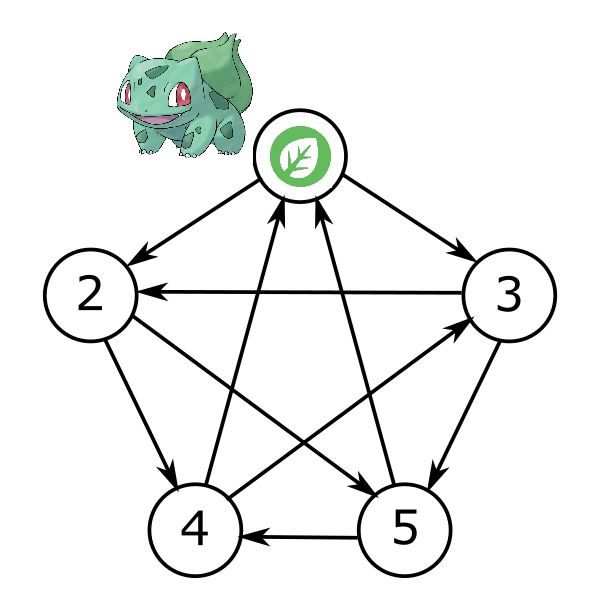
\includegraphics{C:/Users/gadia/Dropbox/Websites/blog/assets/img/2020/08/RPS-5Pokemon-1.PNG}}

עכשיו, מהצומת של בלבאוזר יוצאות שתי קשתות, אל הצמתים {\beginL 2\endL}
ו-{\beginL 3\endL}. המשמעות שאני רוצה שתהיה לקשת \L{$v\overset{e}{\to}u$}
היא \textquotedblright\L{$v$} מנצח את \L{$u$}\textquotedblleft{}
ולכן אני רוצה לשים בצמתים {\beginL 2\endL} ו-{\beginL 3\endL} את הפוקימונים
ש\textquotedblleft עשב\textquotedblleft{} מנצח - במקרה שלנו, הפוקימונים
של \textquotedblright קרקע\textquotedblleft{} ו\textquotedblleft סלע\textquotedblleft .
אז אני אשים אותם שם, אבל צריך להיות זהירים: יש לי \textbf{שתי דרכים}
לעשות את זה. או \textquotedblright{\beginL 2\endL} הופך לסלע, {\beginL 3\endL}
הופך לקרקע\textquotedblleft{} או \textquotedblright{\beginL 2\endL}
הופך לקרקע, {\beginL 3\endL} הופך לסלע\textquotedblleft . האם שתי
הדרכים לגיטימיות? ובכן, לא! כי אני רוצה להמשיך לכבד את היחס \L{$3\to2$}
שמופיע בגרף. מכיוון ש-{\beginL 3\endL} מנצח את {\beginL 2\endL}, גם
מי ש-{\beginL 3\endL} יהפוך אליו צריך לנצח את מי ש-{\beginL 2\endL}
הופך אליו. על פי חוקי הפוקימונים קרקע מנצחת סלע, ולכן {\beginL 3\endL}
יהפוך לפוקימון הקרקע ו-{\beginL 2\endL} יהפוך לפוקימון הסלע:

\L{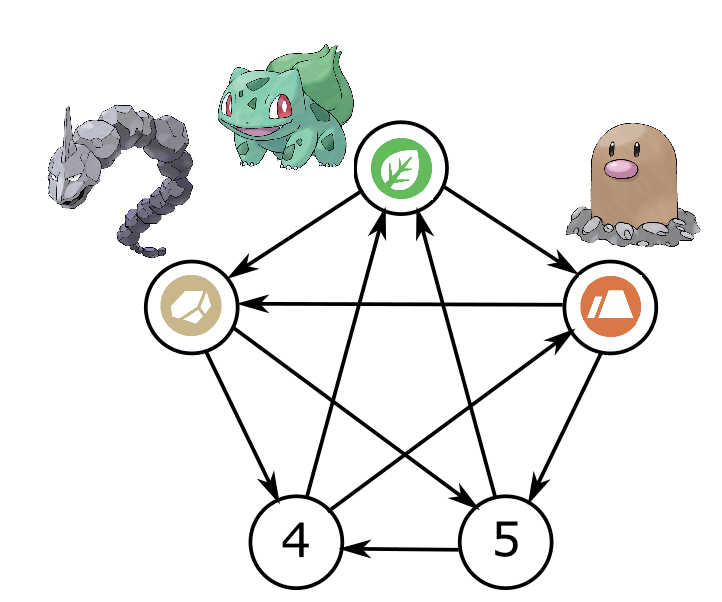
\includegraphics{C:/Users/gadia/Dropbox/Websites/blog/assets/img/2020/08/RPS-5Pokemon-2.PNG}}

עכשיו אפשר להתפנות לשאלה איזה פוקימונים יחליפו את {\beginL 4\endL}
ו-{\beginL 5\endL}. כמו קודם, גם כאן הסתכלות על החצים קובעת לנו מה
חייב להופיע שם: נותרו לנו רק פוקימוני אש וקרח, ועל פי חוקי הפוקימונים
אש מנצחת קרח. מכיוון שהקשת \L{$5\to4$} מראה ש-{\beginL 5\endL} מנצח
את {\beginL 4\endL}, אז בהכרח {\beginL 5\endL} חייב להיות אש ואילו
{\beginL 4\endL} חייב להיות קרח:

\L{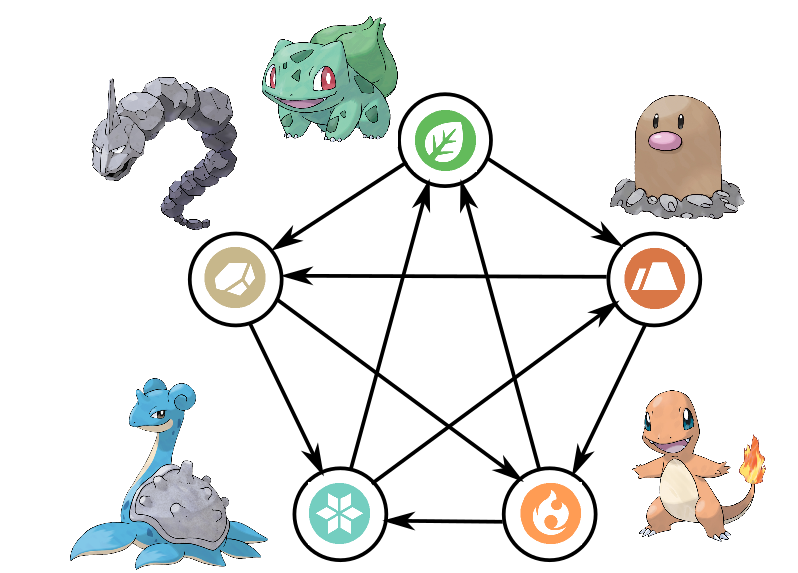
\includegraphics{C:/Users/gadia/Dropbox/Websites/blog/assets/img/2020/08/RPS-5Pokemon-3.PNG}}

זה משלים את הגרף החדש שלנו, אבל שימו לב שאפילו לא בדקתי את כל הקשתות
במפורש. למשל, יש לנו בגרף את הקשת \textquotedblright קרח\L{$\leftarrow$}קרקע\textquotedblleft{}
שלא התייחסתי אליה במפורש. צריך לבדוק שהקשר הזה באמת מתקיים; אבל הדוגמא
שלי הונדסה בקפידה כדי להתאים לחוקים הללו אז אתם יכולים להאמין לי שזה
מתקיים גם בלי לרוץ לחפש מידע באינטרנט על פוקימונים.

בשביל מה זה היה טוב? ראשית, כי פוקימונים זה כיף אז אם אפשר לעשות גרסה
אלטרנטיבית של אבן-נייר-מספריים-לטאה-ספוק עם פוקימונים, למה לא? אבל
שנית, כי רציתי להדגים פה את האופן שבו אנחנו לוקחים את הגרף האבסטרקטי
ו\textquotedblleft מלבישים\textquotedblleft{} עליו בגד נוסף של פוקימונים.
הבגד הזה, מבחינה מתמטית, הוא רק \textbf{סימונים אחרים} לאותו גרף כמו
קודם. וכפי שכבר אמרתי - סימונים אחרים זה חשוב. זה הופך את הגרף למעניין
ויפה, אבל התוכן המתמטי \textbf{זהה}.

כדי לראות את זה, בואו נשים זה לצד זה את שני הגרפים כוכבי הפוסט:

\L{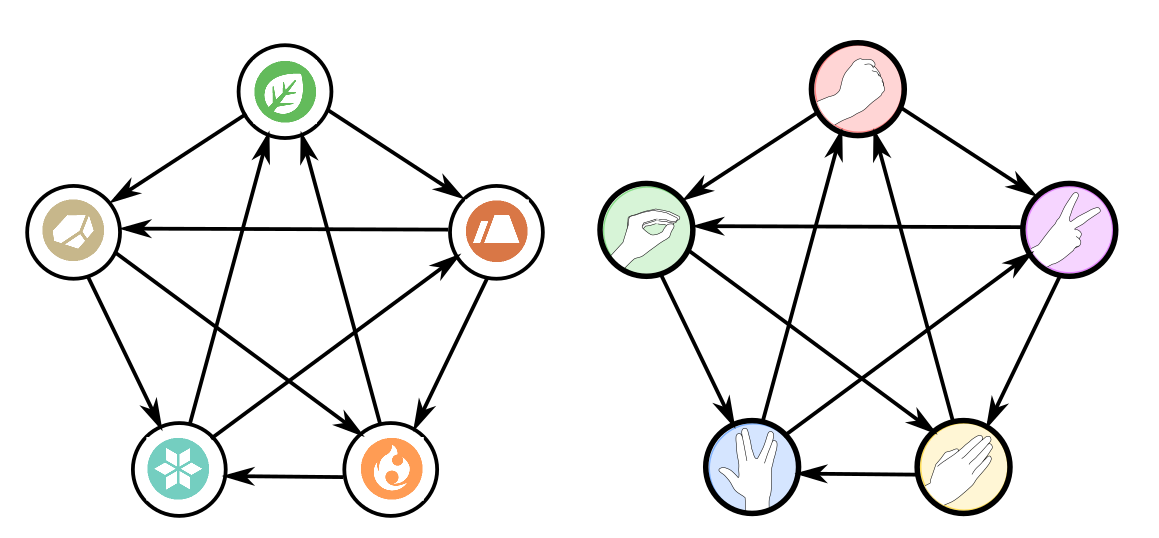
\includegraphics{C:/Users/gadia/Dropbox/Websites/blog/assets/img/2020/08/RPS5-2-Variations.PNG}}

זה לגמרי \textquotedblright אותו הגרף רק עם סימונים שונים\textquotedblleft .
הדרך המתמטית להשתכנע בזה היא בעזרת \textbf{פונקציה} - משהו שמתאים
לכל סימון מהגרף הימני סימון מהגרף השמאלי )יש לי פוסט על פונקציות \L{\href{https://gadial.net/2020/01/12/what_are_functions/}{כאן}}(.
הפונקציה במקרה שלנו היא זו:
\begin{itemize}
\item \textbf{אבן} עוברת אל \textbf{עשב}
\item \textbf{מספריים} עוברים אל \textbf{קרקע}
\item \textbf{נייר} עובר אל \textbf{אש}
\item \textbf{לטאה} עוברת אל \textbf{סלע}
\item \textbf{ספוק} עובר אל \textbf{קרח}
\end{itemize}
הפונקציה שהצגתי כרגע היא מה שנקרא \textquotedblright חד-חד-ערכית ועל\textquotedblleft{}
)יש לי פוסט על פונקציות כאלו \L{\href{https://gadial.net/2020/05/15/invertible_functions/}{כאן}}(.
\textquotedblright חד-חד-ערכית\textquotedblleft{} אומר שאין שני קלטים
לפונקציה שעוברים לאותו פלט )כלומר, לא קורה למשל שגם ספוק וגם לטאה
עוברים אל סלע(. \textquotedblright על\textquotedblleft{} אומר שכל סימן
מהגרף השמאלי באמת מתקבל בתור פלט לאחד מהקלטים. ההגדרות הפורמליות הללו
הן הדרך של המתמטיקה לתפוס את הקונספט של \textquotedblright אותו הדבר
עד כדי שינוי סימונים\textquotedblleft .

במקרה של גרף, יש לנו \textbf{מבנה נוסף} שאנחנו רוצים להתחשב בו - השאלה
\textquotedblright מאיפה לאיפה יש קשת\textquotedblleft . אני רוצה
שאם ניקח שני קלטים \L{$x,y$} מהגרף המקורי כך שיש קשת \L{$x\to y$}
אז תהיה קשת גם מהפלט של \L{$x$} אל הפלט של \L{$y$} - זה מה שהתאמצתי
כל כך לשמור עליו כשבניתי את הגרף של הפוקימונים. בואו נראה איך זה כתוב
פורמלית במתמטית: אם יש לנו \textbf{שני גרפים}, \L{$G_{1}=\left(V_{1},E_{1}\right)$}
ו-\L{$G_{2}=\left(V_{2},E_{2}\right)$}, ויש לנו פונקציה \L{$f:V_{1}\to V_{2}$}
)כלומר, פונקציה שלוקחת קלט ששייך ל-\L{$V_{1}$} ומחזירה פלט ששייך
ל-\L{$V_{2}$}( אנחנו רוצים שיתקיים ש-\L{$u\to v$} מתקיים אם ורק
אם \L{$f\left(u\right)\to f\left(v\right)$} )או קצת יותר פורמלית:
ש-\L{$\left(u,v\right)\in E_{1}$} מתקיים אם ורק אם \L{$\left(f\left(u\right),f\left(v\right)\right)\in E_{2}$}(.

במקרה שבו יש לנו פונקציה \L{$f$} שמקיימת את התנאי הנ\textquotedblleft ל
והיא חד-חד-ערכית ועל, אומרים שהגרפים \L{$G_{1},G_{2}$} הם \textbf{איזומורפיים}
ושהפונקציה \L{$f$} הזו היא \textbf{איזומורפיזם }של הגרפים הללו. המושג
הזה, של איזומורפיזם של גרפים, הוא המושג המתמטי המרכזי שהולך לשחק תפקיד
בכל מה שאני רוצה לדבר עליו בהקשר של אבן-נייר-ומספריים בהמשך.

נקודה אחת ששווה להתייחס אליה היא שהאיזומורפיזם שמצאתי בין גרף הלטאה-ספוק
וגרף הפוקימונים הוא לא האיזומורפיזם \textbf{היחיד} שאפשר למצוא. הייתי
יכול לעשות גם את הדבר הבא:
\begin{itemize}
\item \textbf{אבן} עוברת אל \textbf{סלע} )זה מה שרציתי לעשות מההתחלה! זה
הכי טבעי!(
\item \textbf{מספריים} עוברים אל \textbf{קרח}
\item \textbf{נייר} עובר אל \textbf{קרקע}
\item \textbf{לטאה} עוברת אל \textbf{אש}
\item \textbf{ספוק} עובר אל \textbf{עשב}
\end{itemize}
למעשה, לא קשה לראות שקורה הדבר הבא: אם אני רוצה לבנות איזומורפיזם
בין שני הגרפים, אני יכול לבחור \textbf{איזה צומת שמתחשק לי} ולהעביר
את \textbf{אבן} אליו. מרגע שהעברתי אליו את \textbf{אבן}, כל יתר מה
שהאיזומורפיזם עושה נקבע בלי שתהיה לי שליטה על זה, רק מתוך יחסי ה\textquotedblleft מי
מצביע על מי\textquotedblleft . אם תעברו שוב על התהליך שבו בניתי את
גרף הפוקימונים, זה בדיוק מה שקרה שם: מרגע שקבעתי ש-{\beginL 1\endL}
עובר אל בלבאוזר כבר לא הייתה לי שליטה על המשך התהליך. זה אומר שבסך
הכל יש {\beginL 5\endL} איזומורפיזמים בין הגרפים, אחד לכל פלט אפשרי
של \textquotedblright אבן\textquotedblleft .

לסיום, בואו נגיע אל הפואנטה שלי בפוסט הזה. אמרתי שאיזומורפיזם פירושו
\textquotedblright שני הגרפים הללו הם אותו הדבר עד כדי סימונים\textquotedblleft .
מבחינה מתמטית אבן-נייר-מספריים-לטאה-ספוק הוא \textbf{אותו משחק בדיוק}
כמו משחק הפוקימונים שלי, אפילו אם החוויה שלנו כשאנחנו משחקים במשחקים
היא שונה כי אנחנו אוהבים את ספוק יותר מפוקימונים או ההפך. האם זה \textbf{חייב}
להיות כך? האם כל משחק דמוי אבן-נייר-ומספריים עם {\beginL 5\endL} \textquotedblright נשקים\textquotedblleft{}
יהיה איזומורפי לכל משחק אחר שכזה? התשובה היא \textbf{כן}, ואותו דבר
נכון גם למשחקים עם {\beginL 3\endL} נשקים. אם זה נראה מובן מאליו,
נפלא; האם זה נראה מובן מאליו גם למשחקים עם {\beginL 7\endL} נשקים?
כי בהם התשובה היא \textbf{לא}. יש שלושה משחקים \textbf{שונים} עם {\beginL 7\endL}
נשקים. לא שונים במובן של \textquotedblright סימונים שונים\textquotedblleft{}
אלא שונים במובן של \textbf{לא איזומורפיים}. כלומר, מכאן העסק מתחיל
להסתבך באמת. על זה נדבר בפוסט הבא.
\end{document}
